\documentclass[14pt,aspectratio=169]{beamer}
\setbeamertemplate{caption}[numbered]
\setbeamertemplate{caption label separator}{:}
\setbeamercolor{caption name}{fg=normal text.fg}
\usepackage{amssymb,amsmath}
\usepackage{ifxetex,ifluatex}
\usepackage{fixltx2e} % provides \textsubscript
\usepackage{lmodern}
\ifxetex
  \usepackage{fontspec,xltxtra,xunicode}
  \defaultfontfeatures{Mapping=tex-text,Scale=MatchLowercase}
  \newcommand{\euro}{€}
\else
  \ifluatex
    \usepackage{fontspec}
    \defaultfontfeatures{Mapping=tex-text,Scale=MatchLowercase}
    \newcommand{\euro}{€}
  \else
    \usepackage[T1]{fontenc}
    \usepackage[utf8]{inputenc}
      \fi
\fi
% use upquote if available, for straight quotes in verbatim environments
\IfFileExists{upquote.sty}{\usepackage{upquote}}{}
% use microtype if available
\IfFileExists{microtype.sty}{\usepackage{microtype}}{}
\PassOptionsToPackage{hyphens}{url}
\usepackage{hyperref}
\usepackage{ulem}

% Comment these out if you don't want a slide with just the
% part/section/subsection/subsubsection title:
\AtBeginPart{
  \let\insertpartnumber\relax
  \let\partname\relax
  \frame{\partpage}
}
\AtBeginSection{
  \let\insertsectionnumber\relax
  \let\sectionname\relax
  \begin{frame}[plain]
    \tableofcontents[currentsection]
  \end{frame}
}
\AtBeginSubsection{
  \let\insertsubsectionnumber\relax
  \let\subsectionname\relax
  \frame{\subsectionpage}
}

\setlength{\parindent}{0pt}
\setlength{\parskip}{6pt plus 2pt minus 1pt}
\setlength{\emergencystretch}{3em}  % prevent overfull lines
\setcounter{secnumdepth}{0}
% Thanks Richard Darst on how to get a nice Beamer theme.
% See http://rkd.zgib.net/wiki/DebianBeamerThemes

\usepackage{multicol}
\usepackage{tikz}
\usepackage{ctable}
\usetikzlibrary{positioning}

\usebackgroundtemplate{
\includegraphics[width=\paperwidth]{images/swirl-lightest.pdf}}
\logo{
\includegraphics[viewport=274 335 360 440,width=1cm]{images/openlogo-nd.pdf}}

\definecolor{debianred}{rgb}{.780,.000,.211} % 199,0,54
\definecolor{debianblue}{rgb}{0,.208,.780} % 0,53,199
\definecolor{debianlightbackgroundblue}{rgb}{.941,.941,.957} % 240,240,244
\definecolor{debianbackgroundblue}{rgb}{.776,.784,.878} % 198,200,224

\usetheme{Boadilla}
\setbeamertemplate{navigation symbols}{}

\usecolortheme[named=debianbackgroundblue]{structure}
\setbeamercolor{normal text}{fg=black}
\setbeamercolor{titlelike}{fg=debianblue}
\setbeamercolor{sidebar}{fg=debianred,bg=debianbackgroundblue}

\setbeamercolor{palette sidebar primary}{fg=debianred}
\setbeamercolor{palette sidebar secondary}{fg=debianred}
\setbeamercolor{palette sidebar tertiary}{fg=debianred}
\setbeamercolor{palette sidebar quaternary}{fg=debianred}

\setbeamercolor{section in toc}{fg=debianred}
\setbeamercolor{subsection in toc}{parent=debianred}

\setbeamercolor{item}{fg=debianred}

\setbeamercolor{block title}{fg=debianblue}

\title[Beyond Reproducible builds]{Beyond reproducible builds}
\subtitle{We are not there yet \\
and why "just" achieving reproducible builds \\
won't be enough}
\author[h01ger]{%
   \texorpdfstring{
            \centering
            Debian Reproducible builds team\\
            \href{mailto:reproducible-builds@lists.alioth.debian.org}{reproducible-builds@lists.alioth.debian.org}
   }{h01ger}}
\institute[Debian]{}
\date[hackerspace.gr '15]{%
 hackerspace.gr (Athens, Greece)\\
 \small{2015-12-04}}

\begin{document}

\begin{frame}
 \titlepage
\end{frame}

\begin{frame}
 \frametitle{Debian reproducible builds team}
 \begin{center}
  \begin{columns}
   \small
   \column{.33\linewidth}
    {akira} \\
    {Andrew Ayer} \\
    {Asheesh Laroia} \\
    \only<1>{Chris Lamb}\only<2>{{\color{debianblue} Chris Lamb}} \\
    {Chris West} \\
    {Christoph Berg} \\
    {Daniel Kahn Gillmor} \\
    David Suarez \\
    {Dhole} \\
    Drew Fisher \\
    Esa Peuha \\
    {Guillem Jover} \\
   \column{.33\linewidth}
    Hans-Christoph Steiner \\
    {Helmut Grohne} \\
    \only<1>{Holger Levsen}\only<2>{{\color{debianblue} Holger Levsen}} \\
    \only<1>{Jelmer Vernooij}\only<2>{{\color{debianblue} Jelmer Vernooij}} \\
    {josch} \\
    Juan Picca \\
    \only<1>{Lunar}\only<2>{{\color{debianblue} Lunar}} \\
    Mathieu Bridon \\
    {Mattia Rizzolo} \\
    Nicolas Boulenguez \\
    {Niels Thykier} \\
    Niko Tyni \\
   \column{.33\linewidth}
    {Paul Wise} \\
    Peter De Wachter \\
    Philip Rinn \\
    {Reiner Herrmann} \\
    {Stefano Rivera} \\
    {Stéphane Glondu} \\
    {Steven Chamberlain} \\
    Tom Fitzhenry \\
    Valentin Lorentz \\
    {Wookey} \\
    \only<1>{Ximin Luo}\only<2>{{\color{debianblue} Ximin Luo}} \\
  \end{columns}
 \end{center}
\end{frame}

\begin{frame}
 \frametitle{Who are you?}
 \begin{itemize}
  \item Contributed to Free Software?
  \item<2-3> Seen a talk about reproducible builds this year?
  \item<3> Contributed to this effort?
 \end{itemize}
\end{frame}

\section{About}

\begin{frame}
 \frametitle{The problem}

 \begin{center}
  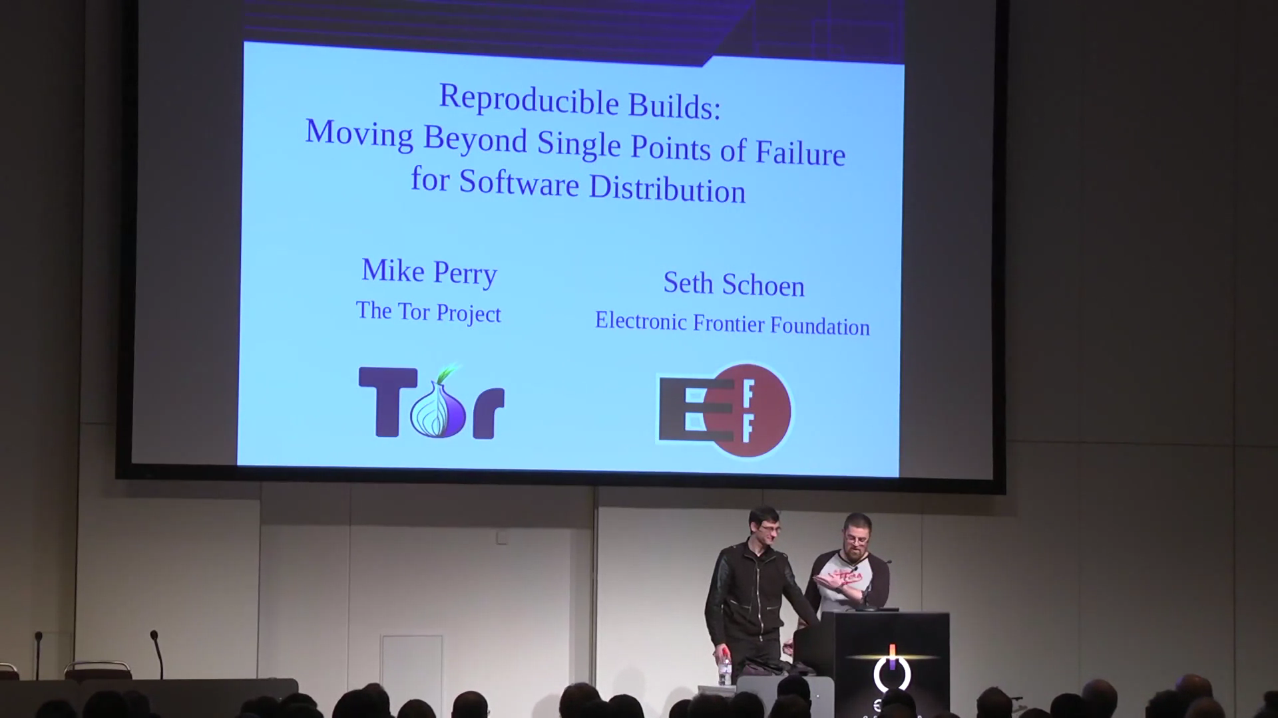
\includegraphics[width=0.7\textwidth]{images/31c3.png}

  Available on \url{media.ccc.de}, 31c3
 \end{center}
\end{frame}

\begin{frame}[fragile]
 \frametitle{A few example's from that 31c3 talk}
 \begin{itemize}
  \item CVE-2002-0083: remote root exploit in \texttt{sshd}, a single bit difference in the binary
  \item 31c3 talk had a live demo with a kernel module modifying source code in memory only
  \item financial incentives to crack developer machines…
  \item how can you be sure what's running on your machine or on a build
  daemon network? Do you ever leave your USB3 ports alone?
 \end{itemize}
\end{frame}

\begin{frame}[fragile]
 \frametitle{Another example from real life}

 At a CIA conference in 2012:
 \begin{center}
  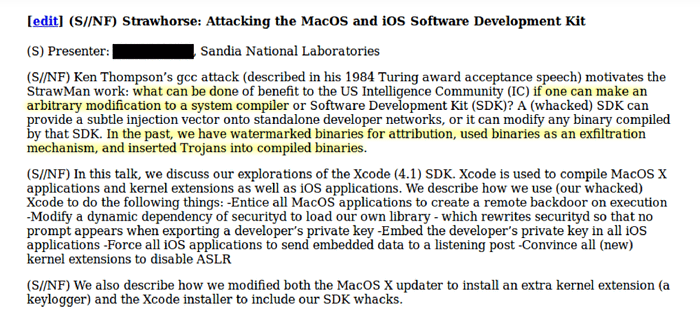
\includegraphics[width=0.8\textwidth]{images/strawhorse.png}

  {\footnotesize
  \url{firstlook.org/theintercept/2015/03/10/ispy-cia-campaign-steal-apples-secrets/}
  }
 \end{center}
\end{frame}


\begin{frame}
 \frametitle{The solution}

 \begin{center}
 \Large{
 Promise that anyone can always generate
 identical binary packages
 from a given source}
\end{center}
\end{frame}


\begin{frame}
 \frametitle{The solution}

 \begin{center}
 We call this:

 \Huge{ “Reproducible builds” }
 \end{center}
\end{frame}

\begin{frame}
 \frametitle{Demo}
% show this once running in plain sid,
% and then in sid with our modified toolchain.
%
% prepare demo:
% mkdir demo ; cd demo ; apt-get source giftrans
%
% do demo:
% PTH=$(mktemp -d); OPTH=$PWD; P=giftrans; cp ${P}_* $PTH/; cd $PTH ;
%   dpkg-source -x ${P}*.dsc ; for X in 1 2 3 4 5 ; do (cd ${P}-*/;
%   dpkg-buildpackage -b -uc -us); mkdir -p .$X ; cp $P_*.deb .$X; done ; rm
%   *.deb ; echo; sha1sum *dsc *z .*/*.deb | grep -v giftrans-dbgsym ; cd - ;
% rm -r $PTH
\end{frame}

\begin{frame}[plain]
\begin{center}
 \Huge{This should become the \textbf{norm}.}

 \visible<2>{\small{ We want to change the meaning of "free software":

  it's only free software if it's reproducible!}}
\end{center}
\end{frame}

\section{Progress}

\begin{frame}[plain]
 \frametitle{Progress in Debian \texttt{unstable}}
 \begin{center}
  \includegraphics[height=0.73\paperheight]{images/stats_pkg_state.png}

  \footnotesize{19,257 out of 23,141 source packages are reproducible \\
    in our test framework}
  \vfill
 \end{center}
\end{frame}


\begin{frame}[plain]
 \frametitle{Progress in the Debian Bug Tracking System (BTS)}
 \begin{tikzpicture}[remember picture,overlay]
  \node[at=(current page.center)] {
    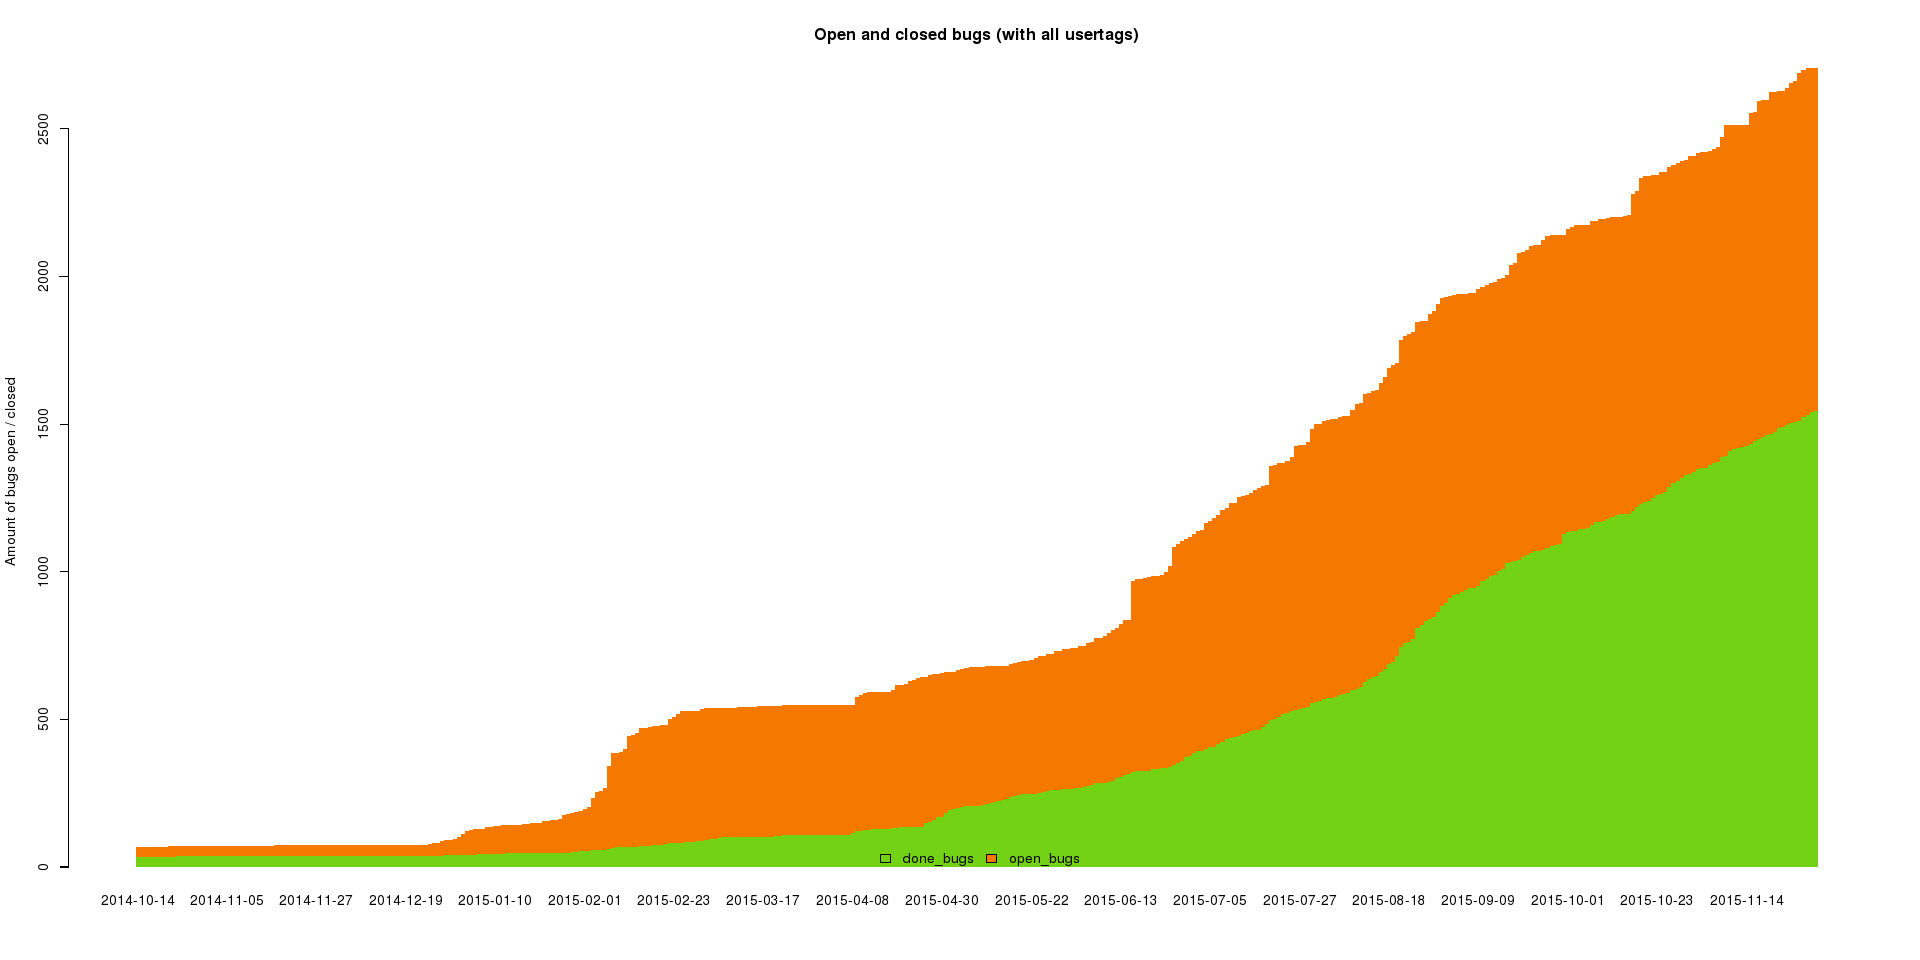
\includegraphics[height=0.73\paperheight]{images/stats_bugs_state.png}
  };
 \end{tikzpicture}
\end{frame}

\begin{frame}
 \frametitle{What we did in Debian since Summer 2014}

 \begin{itemize}
  \item Agreed on using a fixed build path: \texttt{/build/}
  \item Recording the build environment: \texttt{.buildinfo}
  \item \texttt{strip-nondeterminism}
  \item \texttt{reproducible.debian.net}
  \item \texttt{diffoscope} (formerly \texttt{debbindiff})
  \item \texttt{SOURCE\_DATE\_EPOCH}
  \item \texttt{disorderfs}
  \item 700+ patches: \texttt{dpkg}, \texttt{debhelper}, \texttt{sbuild}, …
  \item<2> Tell the world \& collaborate
 \end{itemize}
\end{frame}


\begin{frame}
 \frametitle{Tell the world \& collaborate}

 \begin{itemize}
  \item Recent talks (some available with subtitles):
   \begin{itemize}
    \item 2015-08-13: Chaos Communication Camp 2015
    \item 2015-08-20: DebConf15
    \item 2015-11-08: Mini-DebConf Cambridge 2015
   \end{itemize}
  \item Weekly reports since May 2015
  \item Summit in December 2015 (Athens)
   \begin{itemize}
    \item 40 people from 16 projects
   \end{itemize}
 \end{itemize}
\end{frame}

\begin{frame}
 \frametitle{Tell the world \& collaborate, cont.}

 \begin{itemize}
  \item \texttt{https://reproducible-builds.org}
 \end{itemize}
 \begin{center}
 
\includegraphics[width=0.7\textwidth]{images/rbwww1.png}
 \end{center}
\end{frame}

\begin{frame}
 \frametitle{Stats about reproducible.debian.net}

 \begin{itemize}
  \item Continuously testing Debian testing, unstable and experimental
   \begin{itemize}
    \item \small{ \texttt main only }
    \item \small{ can we build \texttt contrib without legal troubles? }
   \end{itemize}
  \item Also testing coreboot, OpenWrt, NetBSD, FreeBSD,
  Archlinux and soon Fedora
   \begin{itemize}
    \item \small{ those currently only weekly though… }
   \end{itemize}
 \end{itemize}
 \vfill
 \begin{center}
  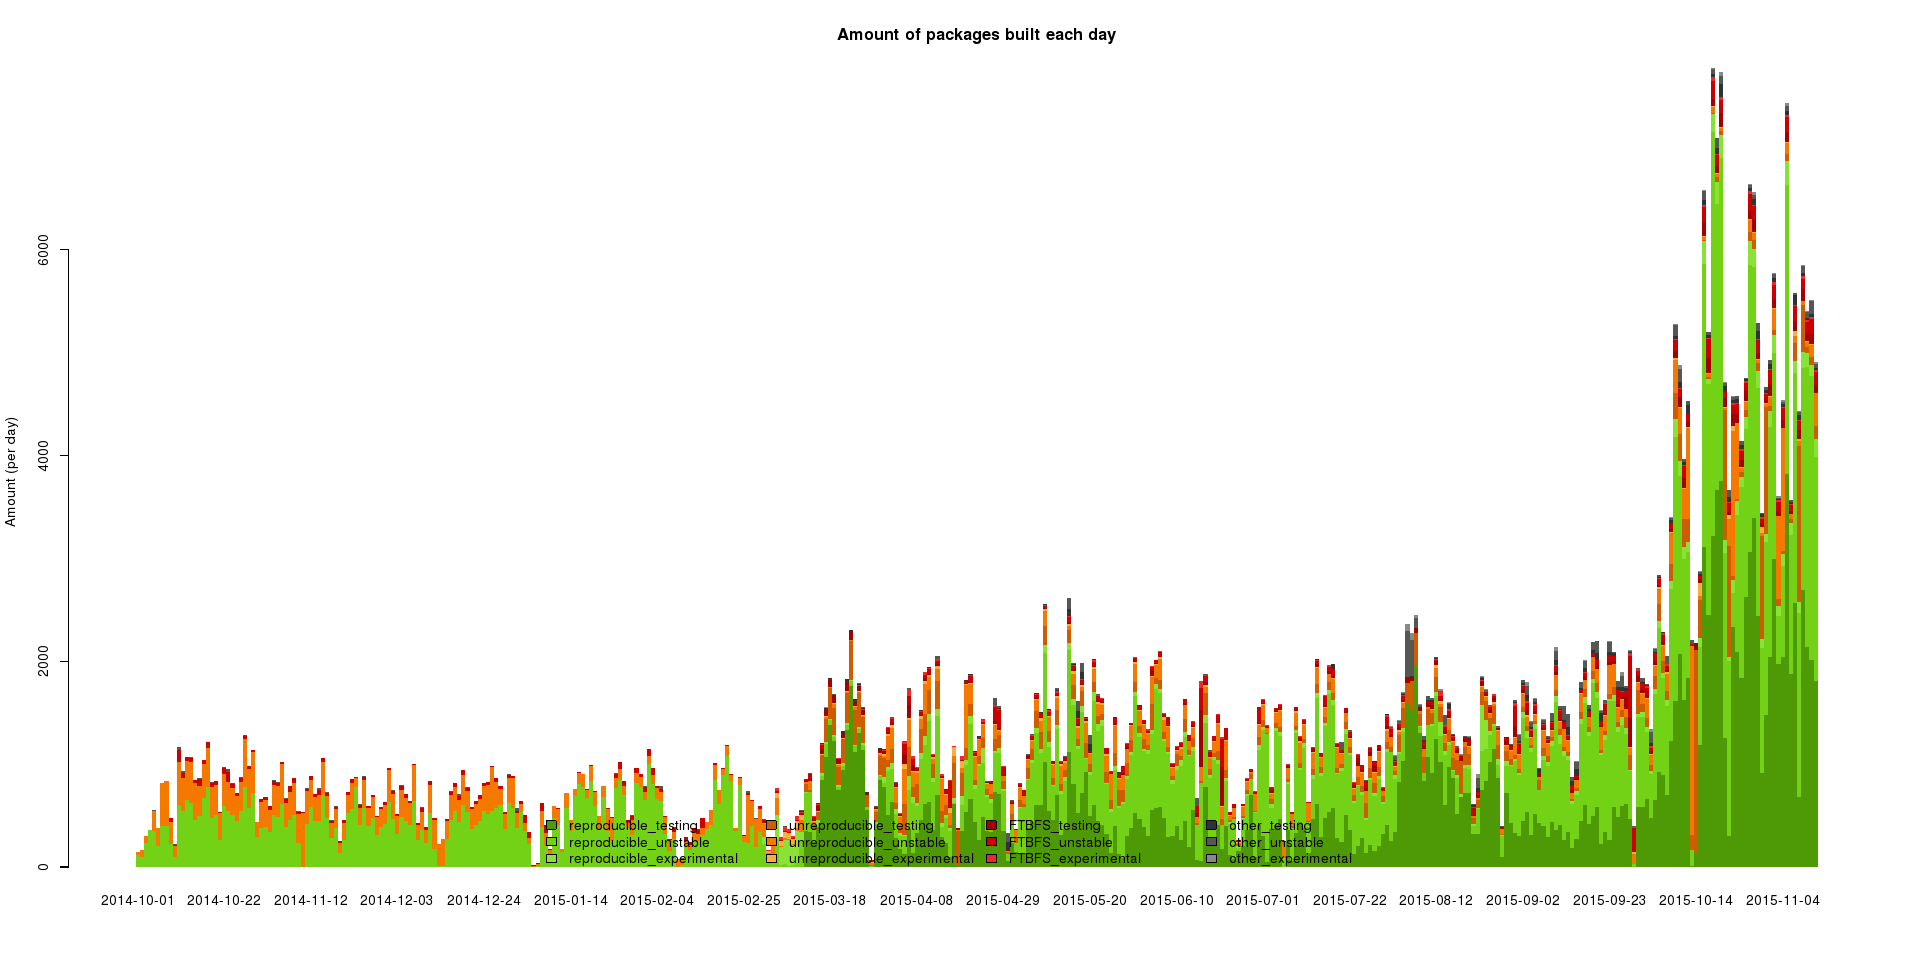
\includegraphics[height=0.47\paperheight]{images/stats_builds_per_day_amd64.png}
 \end{center}
\end{frame}


\begin{frame}
 \frametitle{More stats on reproducible.debian.net}

 \begin{itemize}
  \item 122 jenkins jobs running on 12 hosts
  \item 27 contributors for \texttt{jenkins.debian.net.git}
  \item 4k lines of Python and 5k lines Bash code
  \item \texttt{amd64}: 111 cores and 198 GB RAM split on 9 VMs, provided by
  https://profitbricks.co.uk
  \item \texttt{armhf}: 18 cores and 9 GB RAM on 6 systems, provided by vagrant@d.o.
 \end{itemize}
 \begin{center}
  
\includegraphics[height=0.2\paperheight]{images/profitbricks_logo.png}
  \vfill
 \end{center}
\end{frame}

\begin{frame}
 \frametitle{Good to know about reproducible.debian.net}

 \begin{itemize}
  \item \url {https://reproducible.debian.net/$src}
  \item<2-3> { 165 categorised distinct issues }
  \item<2-3> { 3,496 packages to be fixed in \texttt{sid}, but only 426 without annotated
  issues }
  \item<3> { 29 different "package sets", eg. \texttt{build-essential} is only 78\%
  reproducible
   \begin{center}
    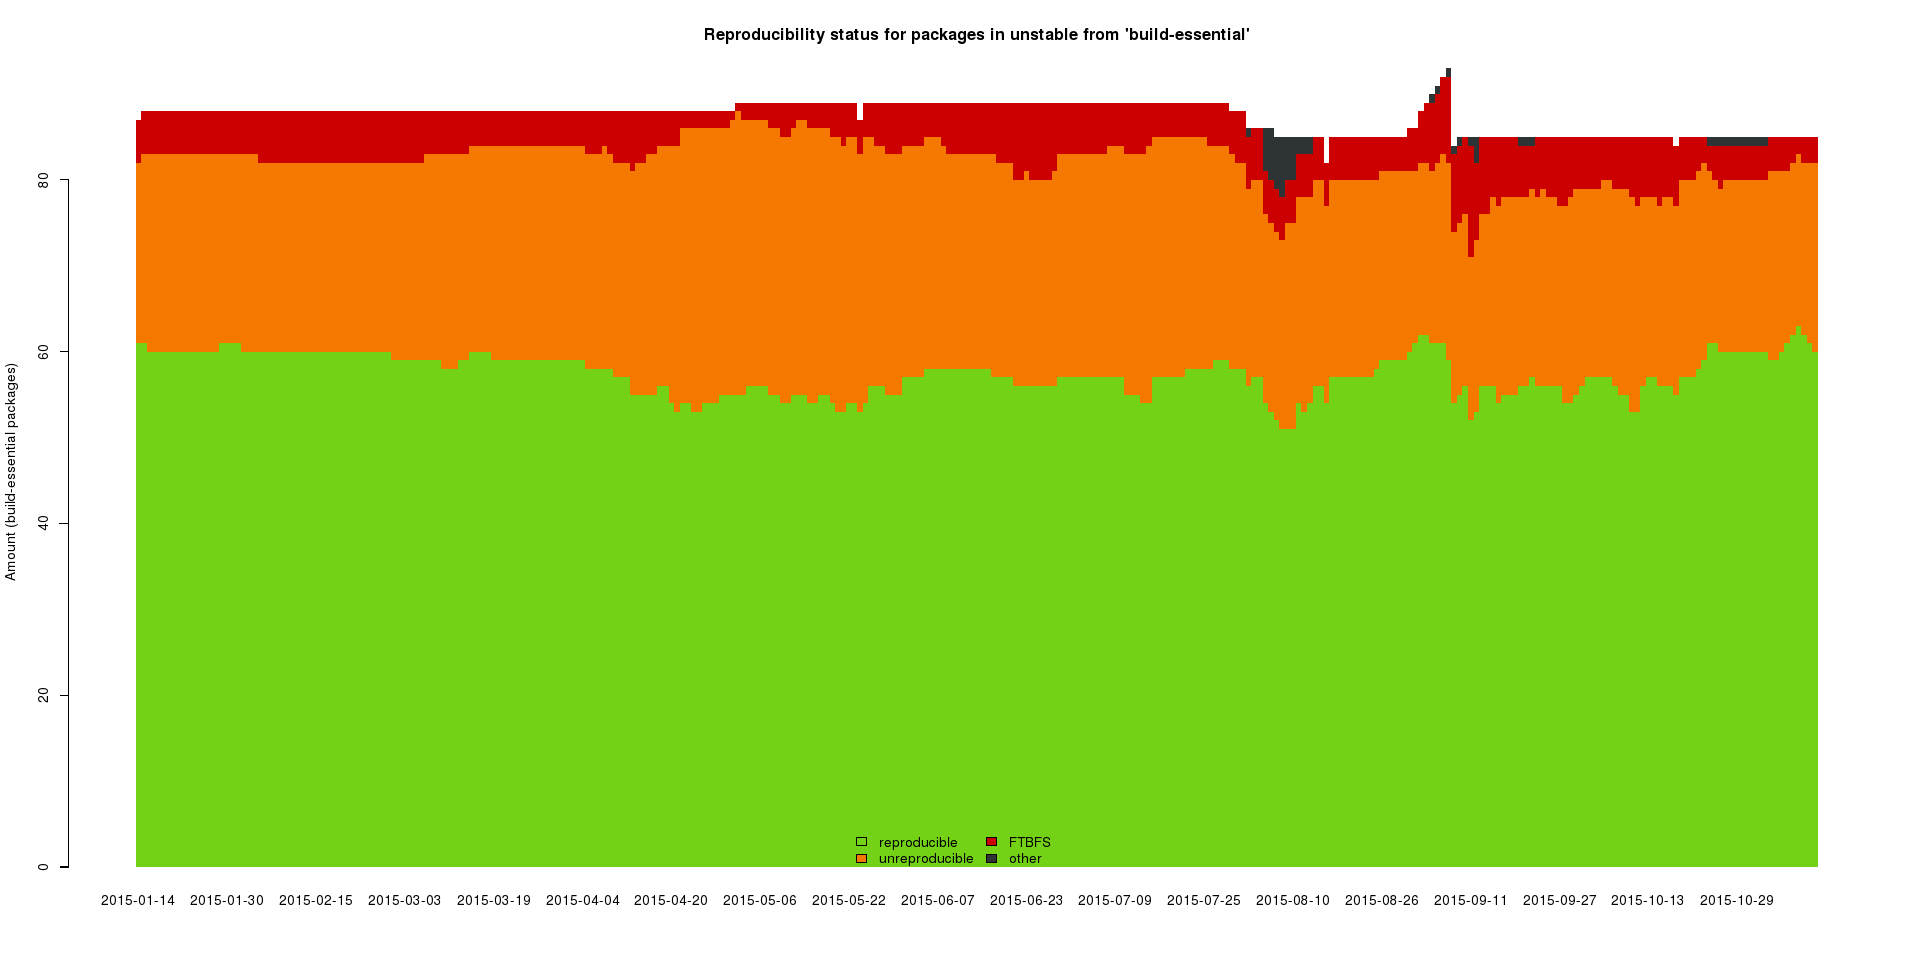
\includegraphics[height=0.5\paperheight]{images/stats_meta_pkg_state_build-essential.png}
   \vfill
 \end{center}
  }
 \end{itemize}
\end{frame}

\begin{frame}
 \frametitle{Future of reproducible.debian.net}

 \begin{itemize}
 \item We want more more more arm(64) cores!
 \end{itemize}
 \begin{center}
  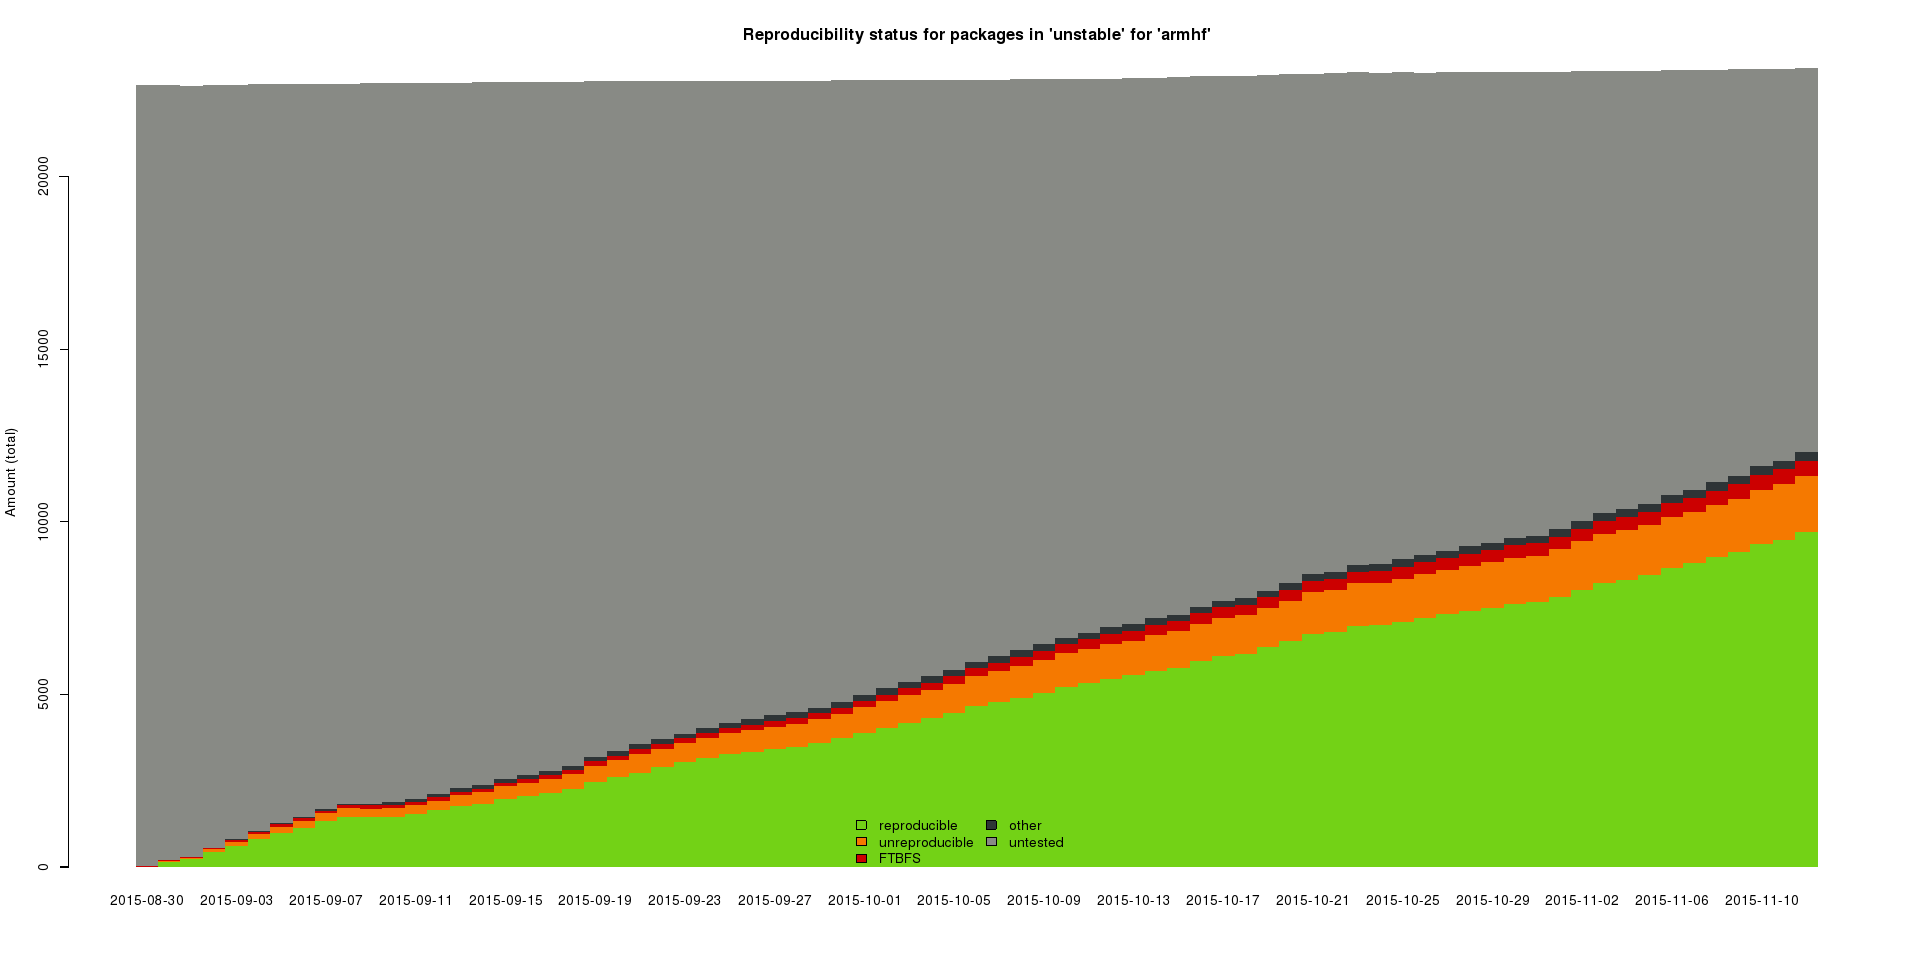
\includegraphics[height=0.73\paperheight]{images/stats_pkg_state_armhf.png}
  \vfill
 \end{center}
\end{frame}


\begin{frame}[fragile]
 \frametitle{Variations on reproducible.debian.net}

 \begin{center}
  \begin{table}
   \resizebox{0.95\textwidth}{!}{%
    \begin{tabular}{l|ll}
\textbf{variation} & \textbf{first build} & \textbf{second build} \\
\hline
hostname & \texttt{jenkins} & \texttt{i-capture-the-hostname} \\
domainname & \texttt{debian.net} & \texttt{i-capture-the-domainname} \\
\texttt{env TZ} & \texttt{GMT+12} & \texttt{GMT-14} \\
\texttt{env LANG} & \texttt{C} & \texttt{fr\_CH.UTF-8} \\
\texttt{env LC\_ALL} & not set & \texttt{fr\_CH.UTF-8} \\
\texttt{env USER} & \texttt{pbuilder1} & \texttt{pbuilder2} \\
uid & \texttt{1111} & \texttt{2222} \\
gid & \texttt{1111} & \texttt{2222} \\
UTS namespace & shared with the host & \textit{modified using \texttt{/usr/bin/unshare --uts}} \\
kernel version & Linux 3.16.0-4 / 4.2.0-0.bpo & Linux 2.6.56-4 / 2.6.62-0.bpo.1 \\
umask & 0022 & 0002 \\
CPU type & \multicolumn{2}{l}{same for both builds \textit{(work in progress)}} \\
filesystem & \multicolumn{2}{l}{same for both builds \textit{(work in progress - disorderfs)}} \\
year, month, date & \multicolumn{2}{l}{same for both builds \textit{(work in progress)}} \\
hour, minute & \multicolumn{2}{l}{hour is usually the same… usually, the minute differs… \textit{(work in progress)}} \\
\textit{everything else} & \multicolumn{2}{l}{\textit{is likely the same…}}
    \end{tabular}
   }
  \end{table}
 \end{center}
\end{frame}



\begin{frame}
 \frametitle{Debian \texttt{.buildinfo} files}

 \begin{itemize}
  \item Aggregates in the same file:
   \begin{itemize}
    \item Sources (checksums)
    \item Generated binaries (checksums)
    \item Packages used to build (with specific version, checksums coming soon)
   \end{itemize}
  \item Can be later used to exactly recreate environment
  \item For Debian, all versions are available from \url{snapshot.debian.org}
 \end{itemize}
\end{frame}


\begin{frame}[fragile]
 \frametitle{Example \texttt{.buildinfo} file}

{\small
\begin{verbatim}
Format: 1.9
Build-Architecture: amd64
Source: txtorcon
Binary: python-txtorcon
Architecture: all
Version: 0.11.0-1
Build-Path: /build/txtorcon-0.11.0-1
Checksums-Sha256:
 a26549d9…7b 125910 python-txtorcon_0.11.0-1_all.deb
 28f6bcbe…69 2039 txtorcon_0.11.0-1.dsc
Build-Environment:
 base-files (= 8),
 base-passwd (= 3.5.37),
 bash (= 4.3-11+b1),
 …
\end{verbatim}
}
\end{frame}



{
\usebackgroundtemplate{%
 \begin{tikzpicture}[remember picture,overlay]%
  \node[shift={(-0.15\paperwidth, 0.4\paperheight)},at=(current page.south east)] {
    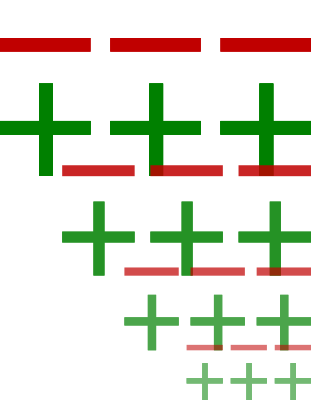
\includegraphics[width=0.2\paperwidth]{images/diffoscope_logo.png}
  };
 \end{tikzpicture}%
}
\begin{frame}{diffoscope}
 \frametitle{Debugging problems: diffoscope}

 \begin{itemize}
  \item Examines differences \textbf{in depth}.
  \item Outputs HTML or plain text with human readable differences.
  \item Recursively unpacks archives, uncompresses PDFs, disassembles
  binaries, unpacks Gettext files, …
  \item Easy to extend to new file formats.
  \item Falls back to binary comparison.
  \item Available from \texttt{git}, PyPI, Debian (sid and stretch), \\
   Arch Linux, Guix, Homebrew.
  \item Maintainers in other distros wanted.
  \item \url{http://diffoscope.org/}
 \end{itemize}
\end{frame}
}

\begin{frame}
 \frametitle{diffoscope example (HTML output)}
 \begin{tikzpicture}[remember picture]
  \node[at=(current page.center)] {
   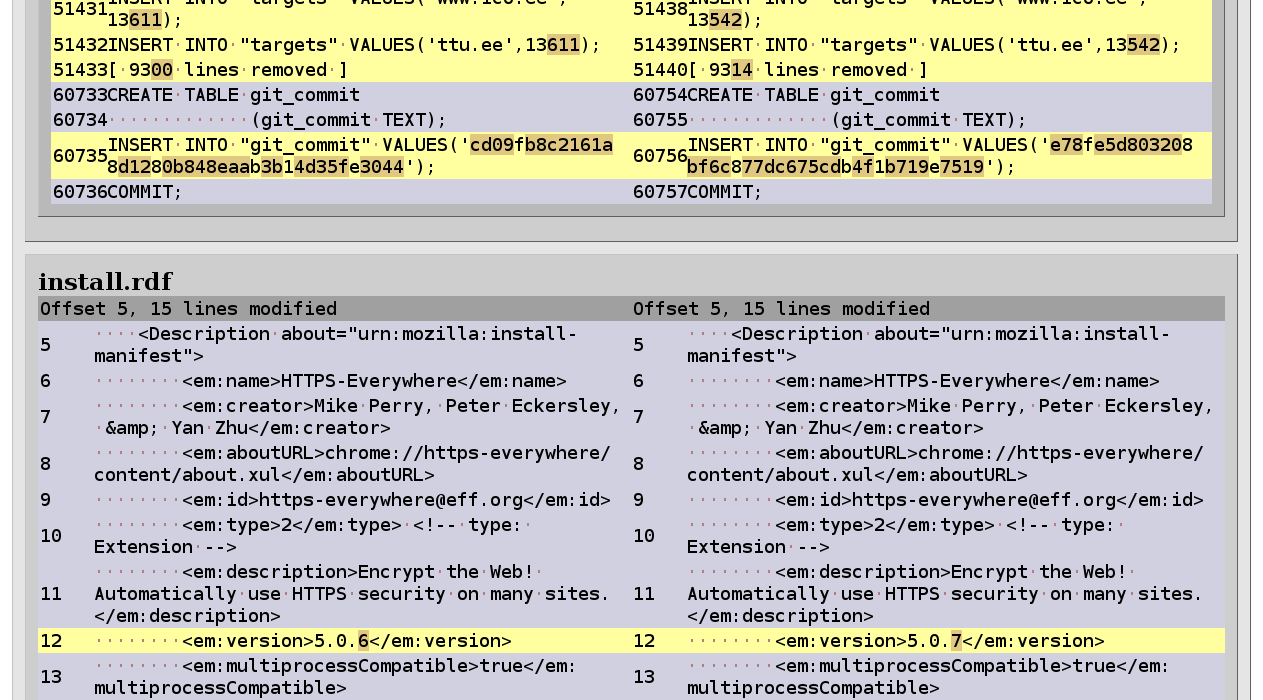
\includegraphics[width=0.9\paperwidth]{images/diffoscope_example_html.png}
  };
 \end{tikzpicture}
\end{frame}

\begin{frame}
 \frametitle{\texttt{diffoscope} is "just" for debugging}

 \begin{itemize}
  \item Reminder: \texttt{diffoscope} is for \textbf{debugging}
  \item<2> "reproducible" according to our definition means: \textbf{bit by bit
  identical}. So the tools for testing whether something is reproducible are
  either \texttt{diff} or \texttt{sha256sum}!
 \end{itemize}
\end{frame}


\begin{frame}
 \frametitle{\texttt{SOURCE\_DATE\_EPOCH}}

 \begin{itemize}
  \item Build date usually not useful for the user
  \item Value of \texttt{SOURCE\_DATE\_EPOCH} instead of current date \& for other seeds
  \item In Debian, set from the latest \texttt{debian/changelog} entry
  \item General solution for other projects \& distributions
 \end{itemize}
\end{frame}

\begin{frame}
 \frametitle{\texttt{SOURCE\_DATE\_EPOCH} (closed bugs)}

 \begin{itemize}
  \item dh-strip-nondeterminism
  \item \sout{\texttt{\#791823}}: debhelper
  \item \sout{\texttt{\#787444}}: help2man
  \item \sout{\texttt{\#790899}}: epydoc
  \item \sout{\texttt{\#794004}}: ghostscript
  \item \sout{\texttt{\#796130}}: man2html
  \item \sout{\texttt{\#783475}}: texi2html
  \item \sout{\texttt{\#794586}}: ocamldoc
  \item \sout{\texttt{\#795942}}: wheel
  \item ...
 \end{itemize}
\end{frame}


\section{Next steps}


\begin{frame}
 \frametitle{\texttt{SOURCE\_DATE\_EPOCH} (open bugs)}

 \begin{itemize}
  \item gcc (\texttt{\_\_DATE\_\_} and \texttt{\_\_TIME\_\_} macros) \texttt{\footnotesize{\url{https://gcc.gnu.org/ml/gcc-patches/2015-06/msg02210.html}}}
  \item \texttt{\#792687, \#804141}: gettext
  \item \texttt{\#792201}: doxygen
  \item \texttt{\#800797}: docbook-utils
  \item \texttt{\#801621}: perl (Pod::Man)
  \item \texttt{\#790801}: txt2man
  \item \texttt{\#791815}: libxslt
  \item \texttt{\#794681}: qt4-x11 (qthelpgenerator)
  \item \texttt{\#792202}: texlive-bin
  \item ...
 \end{itemize}

\end{frame}


\begin{frame}
 \frametitle{Missing bits}
 \begin{itemize}
  \item NB. This is just a proof-of-concept, Debian is not 80\%
  reproducible
  \item Changes still need to be merged
 \end{itemize}
\end{frame}

\begin{frame}
 \frametitle{\texttt{dpkg}}

 \begin{itemize}
  \item \sout{\texttt{\#719844}: make compression of \{data,control\}.tar.gz deterministic}
  \item \texttt{\#759999}: set reproducible timestamps in \texttt{.deb} ar file headers
  \item \texttt{\#787980}: normalize file permissions when creating control.tar
  \item \texttt{\#719845}: make file order within {data,control}.tar.gz deterministic
  \item \texttt{dpkg-genbuldinfo}: \textit{patch already written, but waiting on agreement about spec}
 \end{itemize}
\end{frame}

\begin{frame}
 \frametitle{\texttt{debhelper}}

 \begin{itemize}
  \item \texttt{\#759886}: make mtimes of packaged files deterministic
  \item \sout{\texttt{\#759895}: add a call to
  \texttt{dh\_strip\_nondeterminism} in \texttt{dh}}
  \item \sout{\texttt{\#791823}: set \texttt{SOURCE\_DATE\_EPOCH} env var for
  reproducible builds}
  \item \sout{\texttt{\#802005}: sort file lists passed to 'cp --parents -p'
  for reproducibility}
 \end{itemize}
\end{frame}

\begin{frame}
 \frametitle{\texttt{sbuild}}

 \begin{itemize}
  \item \sout{\texttt{\#790868}: allow sbuild to use a deterministic build
  path to build packages}
  \item \texttt{\#778571}: predictible build location for reproducible builds
  (\texttt{/build})
  \item Finish the \texttt{srebuild} script
 \end{itemize}
\end{frame}

\begin{frame}
 \frametitle{\texttt{ftp.debian.org}}

 \begin{itemize}
  \item \texttt{\#763822}: please include \texttt{.buildinfo} files in the archive
 \end{itemize}
\end{frame}

\begin{frame}
 \frametitle{\texttt{debian-policy}}

 \begin{itemize}
  \item Section 4.15: “Sources \textbf{must} build reproducible binaries.”
  \item<2-3> We hope this will happen after stretch (Debian 9) release
  \item<3> (In 2016: “Sources \textbf{shall} build reproducible binaries.”)
 \end{itemize}
\end{frame}

\section{Beyond building}

\begin{frame}
 \frametitle{Reproducible builds demand a defined build environment}
 \begin{itemize}
  \item Re-creating an identical build environment is mandatory too.
  \item Without an identical build environment, reproducible builds will only
  happen by sheer luck.
  \item<2>{Only solved for Debian right now and currently proof of concept only…}
 \end{itemize}
\end{frame}

\begin{frame}
 \frametitle{Debian release process}
 \begin{itemize}
  \item In our current design and practices, rebuilding stretch will require
  package versions which are not part of stretch.
  \item This design might put a high load on snapshot.debian.org.
  \item<2-4>{Rebuilding all of Debian a month prio the release? }
  \item<3-4>{Cross-builds could even speed up slow archs.}
  \item<4>{More discussions needed. Freeze probably on November 5th 2016.}
 \end{itemize}
\end{frame}

\begin{frame}
 \frametitle{Distributing \texttt{.buildinfo} files}
 \begin{itemize}
  \item Probably 100,000 new files per Debian suite; 50\% increase per suite
  \item Mirrors would not be happy, so should not go there
  \item We'll need more files when we have detached signatures
  \item<2>{Revoking signatures?}
  \item<2>{...}
 \end{itemize}
\end{frame}

\begin{frame}
 \frametitle{Rebuilders and sharing signed checksums}
 \begin{itemize}
  \item Almost no work has been done here yet.
  \item<2-3> Continuous rebuilds should happen in a systematic way and resulting
  checksums properly published.
  \item<3> And then we need a system to sign those checksums and share them. 
 \end{itemize}
\end{frame}

\begin{frame}
 \frametitle{Rebuilders and sharing signed checksums, cont.}
 \begin{itemize}
  \item Individually signed checksums (think web of trust) could work in the
  Debian case (we have a gpg web of trust), but won't scale.
  \item<2-4> { We'll probably could use systematic rebuilders, run by large organisations
  (ACLU, CCC, CERN, DECIX, DESY, Deutsche Bank, EDF, EON, Greenpeace, NASA, NSA, XYZ).}
  \item<3-4> { …and automated installers for those… }
  \item<4> { …and howtos (\texttt {gpg --gen-key})…}
 \end{itemize}
\end{frame}


\begin{frame}
 \frametitle{Integration in user tools}
 \begin{itemize}
  \item "Do you really want to install this unreproducible software (y/N)"
  \item<2-4> "Do you want to build those packages which unconfirmed checksums,
  before installing? (Y/n)"
  \item<3-4>{ "How many signed checksums do you require to call a package
  'reproducible'?"}
  \item<4>{ "Which rebuilders do you want to trust?"}
 \end{itemize}
\end{frame}

\begin{frame}
 \frametitle{Integration in user tools - conclusion}
 \begin{itemize}
  \item "Rebuilders and sharing signed checksums" needs to be designed
  (and probably at least partly implemented) before thinking more about
  user tools. It's just clear we need them. 
 \end{itemize}
\end{frame}

\section{Want to help?}

\begin{frame}
 \frametitle{As a developer}
 \begin{itemize}
  \item Stop using build dates
  \item Use \texttt{SOURCE\_DATE\_EPOCH} instead
  \item See \url{https://reproducible-builds.org/specs/}
 \end{itemize}
\end{frame}

\begin{frame}
 \frametitle{Get involved - learning by doing}

 \begin{itemize}
  \item Test for yourself:
   \begin{itemize}
    \item Build something twice, run diffoscope on the results
    \begin{itemize}
     \item For better results use our “reproducible” repository, \texttt{pbuilder} and a custom config
    \end{itemize}
   \end{itemize}
  \item Docs on the web: \\
    \small{\url{https://reproducible-builds.org/docs/}} \\
    \small{\url{https://wiki.debian.org/ReproducibleBuilds/ExperimentalToolchain}}
  \item Ask for help on \texttt{\#debian-reproducible} or on mailing list
 \end{itemize}
\end{frame}

\begin{frame}
 \frametitle{Join the team!}

 \begin{itemize}
  \item Why?
   \begin{itemize}
    \item \heartsuit{}\heartsuit{}\heartsuit{} Lovely group of people \heartsuit{}\heartsuit{}\heartsuit{}
    \item Learn something new everyday
    \item Change the (software) world!
   \end{itemize}
  \item What do we do?
   \begin{itemize}
    \item Review packages
    \item Identify issues and document solutions
    \item \texttt{reproducible.d.n}, diffoscope, strip-nondeterminism
    \item Propose changes for toolchain
    \item Submit patches for individual packages
    \item Write more general documentation and talk to the world
   \end{itemize}
 \end{itemize}
\end{frame}

\begin{frame}
 \frametitle{Create a new team!}

 \begin{itemize}
  \item Why?
   \begin{itemize}
    \item Every distribution should be reproducible!
    \item Learn something new everyday
    \item Change the (software) world!
   \end{itemize}
  \item How to get started?
   \begin{itemize}
    \item Talk to me here or talk to us on IRC or via mail.
    \item RTFM, there is lots of documentation
    \item Experiment - learning by doing
   \end{itemize}
 \end{itemize}
\end{frame}


\begin{frame}
 \frametitle{Help migrating to \texttt{.debian.org} infrastructure}

 \begin{itemize}
  \item DSA would give us more build nodes of other architectures
  \item \texttt{sudo pbuilder} doesn't make Debian SysAdmins (DSA) happy
  \item Maintenance script really makes DSA unhappy. (\texttt{sudo kill -9 *}..)
  \item<2-3> \texttt{jenkins.debian.org} migration
  \item<3> No prior involvement in Debian needed.
 \end{itemize}
\end{frame}

\section{Questions, comments, ideas?}


\begin{frame}
 \frametitle{Questions, comments, ideas?}

 \begin{itemize}
  \item \url{https://reproducible-builds.org}
  \item \url{https://reproducible.debian.net}
  \item \texttt{\#debian-reproducible} on \texttt{irc.OFTC.net}
 \end{itemize}
\end{frame}


\begin{frame}
 \frametitle{Thanks!}

 \begin{itemize}
  \item Debian “Reproducible Builds” team \\
        {\small (you are just \textbf{so} awesome!)}
  \item Linux Foundation and the Core Infrastructure Initiative
\end{itemize}

 \begin{center}
  
\includegraphics[height=0.1\paperheight]{images/linux_foundation_logo.png}
  \hspace{0.1\paperwidth}
  
\includegraphics[height=0.1\paperheight]{images/cii_logo.png}
 \end{center}

 \vfill
 \begin{center}
  \resizebox{0.8\textwidth}{!}{%
   \begin{tabular}{rl}
    \texttt{holger@debian.org} & \texttt{B8BF 5413 7B09 D35C F026} \\
                               & \texttt{FE9D 091A B856 069A AA1C} 
   \end{tabular}
  }
 \end{center}
\end{frame}

\end{document}
